%Dokumentklasse

%draft als optionohne bilder für bessere performance
%\documentclass[a4paper,12pt,]{scrreprt}

%normal mit Bildern
\documentclass[
a4paper,
12pt,
draft=True]
{scrartcl}

%angepasster \today Command
\newcommand{\leadingzero}[1]{\ifnum #1<10 0\the#1\else\the#1\fi}
\newcommand{\todayDE}{\leadingzero{\day}.\leadingzero{\month}.\the\year}

%Section als Chapter
\RedeclareSectionCommand[%
%beforeskip = -1sp plus -1sp minus -1sp,% kleinster negativer Wert, um den Absatzeinzug nach der Überschrift zu verhindern.
afterskip = 1.5 \baselineskip plus -1sp minus 1sp,
font = \Huge,
]{section}

\usepackage[left= 3cm,right = 3cm, bottom = 3cm,top = 3cm]{geometry}
%\usepackage[onehalfspacing]{setspace}

% ============= Packages =============
% Dokumentinformationen
\usepackage[
pdftitle={Praktikum - Umwelttechnik},
pdfsubject={},
pdfauthor={Roman-Luca Zank},
pdfkeywords={},	
%Links nicht einrahmen
hidelinks
]{hyperref}

%nur Text zum prüfen des Umfangs

% Standard Packages
%\usepackage[bottom]{footmisc}
\usepackage[utf8]{inputenc}
\usepackage[ngerman]{babel}

\usepackage[T1]{fontenc}
%\usepackage{helvet}

%\renewcommand{\familydefault}{\sfdefault}

\usepackage{colortbl}
\usepackage{graphicx}
\graphicspath{{img/}}
\usepackage{mhchem}
\usepackage{fancyhdr}
\usepackage{lmodern}
\usepackage[table]{xcolor}
\usepackage{placeins}
\usepackage{booktabs}
\usepackage{caption}
\usepackage[list=true]{subcaption}
\usepackage{longtable}
\usepackage{tikz}
\usepackage{pgfplots}
\pgfplotsset{/pgf/number format/use comma}
\pgfplotsset{grid style={white!90!black}}
\usepackage{lastpage}
%\usepackage{ulem}
\usepackage{mathtools}
\usepackage{adjustbox}
\usetikzlibrary{patterns}
\usepackage{pdfpages}
\usepackage[shortlabels]{enumitem}

%Einheitenpackage
\usepackage{siunitx}  
\sisetup{	locale = DE, 
	per-mode=fraction,
	inter-unit-product=\ensuremath{\cdot},
	detect-weight = true,
	quotient-mode=fraction
}
%neue Einheiten definieren
\DeclareSIUnit\xyz{xyz}	
\DeclareSIUnit\rpm{rpm}	
\DeclareSIUnit\mws{mWS}	
\DeclareSIUnit\degrees{^\circ}	

%Automatisch cdot statt *
\DeclareMathSymbol{*}{\mathbin}{symbols}{"01}


%Tabelle
\usepackage{tabularx}
\usepackage{tabulary}

%nur letzte Zeile der Gleichung nummerieren
\makeatletter
\def\Let@{\def\\{\notag\math@cr}}
\makeatother

% zusätzliche Schriftzeichen der American Mathematical Society
\usepackage{amsfonts}
\usepackage{amsmath}

%Abkürzungsverzeichnis
\usepackage{acronym}

%kein Abstand bei neuem Kapitel vom Seitenanfang
%\vspace*{2.3\baselineskip} = ORIGINAL
%\renewcommand*{\chapterheadstartvskip}{\vspace*{.0\baselineskip}}

%nicht einrücken nach Absatz
\setlength{\parindent}{0pt}


\urlstyle{same}

% ============= Kopf- und Fußzeile =============
\pagestyle{fancy}
%
\lhead{}
\chead{}
\rhead{}%\slshape }%\leftmark}
%%
\lfoot{}
\cfoot{}
\rfoot[{\thepage\ of \pageref*{LastPage}}]{Seite \thepage\ von \pageref*{LastPage}}
%%
\renewcommand{\headrulewidth}{0pt}
\renewcommand{\footrulewidth}{0pt}
%\renewcommand{\chapterpagestyle}{fancy}

%Fußnotelinie
%\let\footnoterule

%Fußnote mit Klammer
\renewcommand*{\thefootnote}{(\arabic{footnote})}

%Abb. statt Abbildung
\addto\captionsngerman{%
	\renewcommand{\figurename}{Abb.}%
	\renewcommand{\tablename}{Tab.}%
}

% ============= Package Einstellungen & Sonstiges ============= 
%Besondere Trennungen
%\hyphenation{De-zi-mal-tren-nung}
\usepackage[none]{hyphenat}
\hyphenpenalty=5000
\tolerance=5000
\providecommand\phantomsection{}

\usepackage{mathtools}


% ============= Dokumentbeginn =============

\begin{document}
%Seiten ohne Kopf- und Fußzeile sowie Seitenzahl
\pagestyle{empty}

%\begin{center}
	\begin{tabular}{p{\textwidth}}
		
		
		\begin{center}
			
\includegraphics[scale=0.75]{logos.jpg}\\
		\end{center}
		
		
		\\
		
		\begin{center}
			\LARGE{\textsc{
					Protokoll \\
					Physikalische Chemie\\
			}}
		\end{center}
		
		\\
		
		%\begin{center}
		%\large{Fakultät für Muster und Beispiele \\
		%der Hochschule Musterhausen \\}
		%\end{center}
		%
		%\\
		
		\begin{center}
			\textbf{\Large{Untersuchungen zur Dampfdruckkurve einer reinen Flüssigkeit mittels Ebulliometrie}}
		\end{center}
		
		\begin{center}
			\large{Gruppe 3.2 (BCUC4)}
		\end{center}
		
		
		\\
		%\begin{center}
		%zur Erlangung des akademischen Grades\\
		%Bachelor of Engineering
		%\end{center}
		
		
		%\begin{center}
		%vorgelegt von
		%\end{center}
		
		\begin{center}
			\Large{\textbf{Teilnehmer:}} \\ 
		\end{center}
		\begin{center}
			\large{Roman-Luca Zank}
		\end{center}
		
		
		\\
		
		\begin{center}
			\begin{tabular}{lll}
				\large{\textbf{Protokollführer:}} & &  \large{Roman-Luca Zank}\\
				&&\\
				\large{\textbf{Datum der Versuchsdurchführung:}}&& \large{25.06.2020}\\
				&&\\
				\large{\textbf{Abgabedatum:}}&& \large{\today}\\
				&&\\
				\large{\textbf{Status:}}&& \large{Erstabgabe}\\
			\end{tabular}
		\end{center}
		
		\\ \\ \\ \\ \\ \\ \\ 
		\large{Merseburg den \today}
		
	\end{tabular}
\end{center}


%\include{14_danksagungen}

%\include{15_zusammenfassung}

% Beendet eine Seite und erzwingt auf den nachfolgenden Seiten die Ausgabe aller Gleitobjekte (z.B. Abbildungen), die bislang definiert, aber noch nicht ausgegeben wurden. Dieser Befehl fügt, falls nötig, eine leere Seite ein, sodaß die nächste Seite nach den Gleitobjekten eine ungerade Seitennummer hat. 
\cleardoubleoddpage

% Pagestyle für Titelblatt leer
\pagestyle{empty}

%Seite zählen ab
\setcounter{page}{0}

%Titelblatt
\begin{center}
	\begin{tabular}{p{\textwidth}}
		
		
		\begin{center}
			
\includegraphics[scale=0.75]{logos.jpg}\\
		\end{center}
		
		
		\\
		
		\begin{center}
			\LARGE{\textsc{
					Protokoll \\
					Physikalische Chemie\\
			}}
		\end{center}
		
		\\
		
		%\begin{center}
		%\large{Fakultät für Muster und Beispiele \\
		%der Hochschule Musterhausen \\}
		%\end{center}
		%
		%\\
		
		\begin{center}
			\textbf{\Large{Untersuchungen zur Dampfdruckkurve einer reinen Flüssigkeit mittels Ebulliometrie}}
		\end{center}
		
		\begin{center}
			\large{Gruppe 3.2 (BCUC4)}
		\end{center}
		
		
		\\
		%\begin{center}
		%zur Erlangung des akademischen Grades\\
		%Bachelor of Engineering
		%\end{center}
		
		
		%\begin{center}
		%vorgelegt von
		%\end{center}
		
		\begin{center}
			\Large{\textbf{Teilnehmer:}} \\ 
		\end{center}
		\begin{center}
			\large{Roman-Luca Zank}
		\end{center}
		
		
		\\
		
		\begin{center}
			\begin{tabular}{lll}
				\large{\textbf{Protokollführer:}} & &  \large{Roman-Luca Zank}\\
				&&\\
				\large{\textbf{Datum der Versuchsdurchführung:}}&& \large{25.06.2020}\\
				&&\\
				\large{\textbf{Abgabedatum:}}&& \large{\today}\\
				&&\\
				\large{\textbf{Status:}}&& \large{Erstabgabe}\\
			\end{tabular}
		\end{center}
		
		\\ \\ \\ \\ \\ \\ \\ 
		\large{Merseburg den \today}
		
	\end{tabular}
\end{center}
 %Prokolle
%\begin{center}
\begin{tabular}{p{\textwidth}}


\begin{center}

\includegraphics[scale=0.75]{img/logos.jpg}\\
\end{center}


\\

\begin{center}
\LARGE{\textsc{
Recherche \\
Rückgewinnung von Ammoniak aus Industrieabwässern\\
}}
\end{center}

%\begin{center}
%\large{Fakultät für Muster und Beispiele \\
%der Hochschule Musterhausen \\}
%\end{center}
%
%\\
 \\
 
\begin{center}
\textbf{\Large{Seminararbeit in Medienrecherche}}
\end{center}

\begin{center}
	\large{im WiSe 2019}
\end{center}
 \\
%\begin{center}
%zur Erlangung des akademischen Grades\\
%Bachelor of Engineering
%\end{center}


\begin{center}
\large{vorgelegt von}
\end{center}
\\


\begin{center}
\Large{\textbf{Roman-Luca Zank}} \\
\end{center}

\begin{center}
3. Semester \\
Chemie- und Umwelttechnik \\
\end{center}


\begin{center}
\begin{tabular}{lll}
	\textbf{E-Mail:} & & romanzank@mail.de\\
	\textbf{Matrikelnummer:} & &25240\\
	\textbf{Adresse:} & &Platz der Bausoldaten 2, Zimmer 224\\
	\textbf{Ort:} & &06217 Merseburg\\
	&& \\
	\textbf{Prüfer:} & & Dr. Frank  Baumann\\
\end{tabular}
\end{center}

\\ \\ \\ \\ \\
\large{Merseburg, \today}

\end{tabular}
\end{center}
 %Seminar-/Abschlussarbeit

% Pagestyle für Rest des Dokuments
\pagestyle{fancy}

%Inhaltsverzeichnis
\tableofcontents
\thispagestyle{empty}
\newpage

%Inhalt
%
%Verzeichnis aller Bilder
\label{sec:bilder}
\listoffigures
\addcontentsline{toc}{chapter}{Abbildungsverzeichnis}
\thispagestyle{empty}

%Verzeichnis aller Tabellen
\label{sec:tabellen}
\listoftables
\addcontentsline{toc}{chapter}{Tabellenverzeichnis}
\thispagestyle{empty}



%%Abkürzungsverzeichnis
%\setlength{\columnsep}{20pt}
%\twocolumn
%\addchap{Nomenklatur}
%\label{sec:abkurzung}
%\begin{acronym}
%\acro{kf}[$\text{k}_\text{f}$]{Durchlässigkeitsbeiwert}
%\acro{t}{Durchlaufzeit}
%\acro{tm}[$\text{t}_\text{m}$]{Mittlere Durchlaufzeit}
%\acro{V}{Volumen}
%\acro{h}{Höhe der Wassersäule}
%\acro{Q}{Volumenstrom}
%\acro{l}{Durchströmte Länge}
%\acro{A}{Grundfläche}
%\acro{d}{Durchmesser}
%
%\end{acronym}
%\subsubsection{Aufrufen einer Abkürzung}
%\acs{rT}
%\begin{verbatim}
%\acs{Abkürzung}
%\end{verbatim}

\section{Einleitung und Versuchsziel}
\label{sec:aufgabenstellung}
%- Darstellung des Versuchsziels und der in dem Versuch bearbeiteten Fragestellungen.
%- Kurze Einführung grundlegenden theoretischen Zusammenhänge und der
%Gleichungen die für den Versuch und die Versuchsauswertung relevant sind.
%- Alle Abbildungen sind durchzunummerieren (Abb. 01, …) und mit einer Bild- bzw.
%Tabellenunterschrift zu versehen. Externe Quellen sind in der Bildunterschrift als
%Literatur-Nummer (Quelle: [1]) oder Literatur-Kürzel (Quelle: [Schmidt2015])
%anzugeben.Physikalische Chemie
%FB Ingenieur- und Naturwissenschaften
%Protokollvorlage PC-II Praktikum, SoSe 2020 2
%- Alle Formeln sind durchzunummerieren.
%- Benennung der experimentellen Geräte und Hilfsmittel mit denen der Versuch
%durchgeführt wird (Bsp: Thermostat Firma/Typ XY, Druckmessröhre Firma/Typ Z).

Im Praktikumsversuch "`Oberflächenspannung an Grenzflächen"' werden verschiedene, wässrige Proben auf ihre Oberflächenspannung untersucht. Zudem ist die Temperaturabhängigkeit der Oberflächenspannung mit Hilfe von Wasser zu analysieren.\\
Die Vorgänge an Grenzflächen  sind von großer Bedeutung für Prozesse mit Phasenwechsel. Um diese charakterisieren und weitere rechnerische Vorhersagen treffen zu können, ist die Oberflächenspannung ein entscheidender Bestandteil für diese Beschreibungen.

\section*{Theoretische Grundlagen}
\subsection*{Kohäsions- und Adhäsionskräfte}
Zwischen Teilchen in einer flüssigen Phasen herrschen Wechselwirkungskräfte. Diese sind bedingt durch Anziehungskräfte der Teilchen untereinander in der Flüssigkeit. Für homogen verteilte Teilchen innerhalb der flüssigen Phase resultiert, aufgrund der geringen Reichweite dieser Kräfte, eine Gesamtkraft von null. Betrachtet man die Teilchen, welche sich direkt an der Phasengrenze der Flüssigkeit befinden, so ist dieser zuvor beschriebene Zusammenhang ungültig. Da auf diese Grenzteilchen, auch \textsc{Bulk}-Teilchen genannt, auch Kräfte aus der benachbarten Phase und nicht nur aus der eigenen Phase wirken, können hier resultierende Kräfte größer  oder kleiner null sein. Diese resultierende Kraft steht in diesem Fall senkrecht zur Grenzfläche.\linebreak
Im Folgenden wird für die Beschreibung von Kräften innerhalb der stoffeigenen Phase von Kohäsions- und Kräften zwischen Phasen von Adhäsionskräften gesprochen. Sind die Adhäsionskräfte signifikant größer als die Kohäsionskräfte so maximiert die betrachtete Flüssigkeit ihre Oberfläche der Grenzschicht. Die resultierende Kraft wirkt hierbei entgegensetzt zum Phaseninneren der Flüssigkeit. Wirkt die resultierende Kraft in das Phaseninnere so sind die Kohäsionskräfte größer als die Adhäsionskräfte und die Grenzfläche der Flüssigkeit ist versucht ihre Oberfläche zu minimieren.

\subsection*{Ringmethode nach \textsc{Du Noüy}}
Die Abreißmethode nach \textsc{Du Noüy} wird zur Bestimmung von Oberflächenspannungen von $v$-$l$- sowie $l$-$l$-Systemen genutzt. Bei dieser Methode wird mittels Torsionswaage  die wirkende Kraft beim langsamen Herausziehen eines Platin-Iridium-Ringes, welcher in die Flüssigkeit eingetaucht wird. Die wirkende Kraft am Ring wird nun solang erhöht bis die Benetzung der Flüssigkeit abreißt. Die letzte maximal wirkende Kraft entspricht dann der Oberflächenspannung.
\newpage
Das angehobene Flüssigkeitsvolumen durch Ring und Torsionswaage wirkt dabei der angelegten Kraft am Ring entgegen. Für die Oberflächenspannung ergibt sich dann:
\begin{flalign}
\label{gl:zyl}
	\sigma	&= \frac{F_{\text{max}}}{4*\pi *R_{\text{mittel}}}
\end{flalign}
Zu beachten gilt es, dass für die Gleichung \eqref{gl:zyl} die Annahme getroffen, dass ein idealer Zylinder angehoben wird. In der Realität zeigt sich, jedoch ein gekrümmtes Volumen, welches in die Berechnung mit einbezogen werden muss (siehe Abb. \ref{fig:ring_real}). 
\begin{figure}[h!]
	\centering
	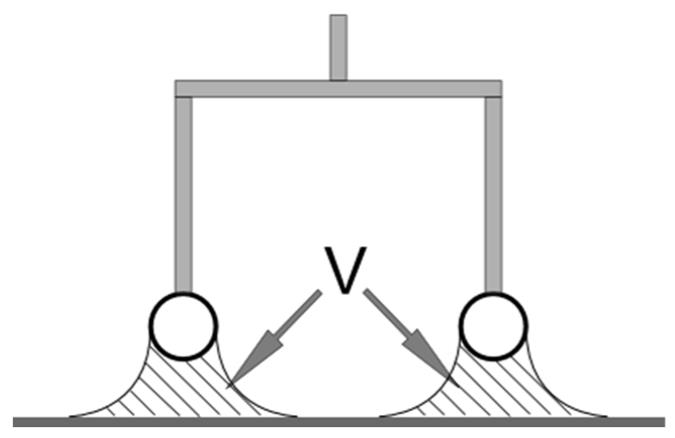
\includegraphics[width=0.5\textwidth]{img/real}
	\caption{Schematische Darstellung des tatsächlich angehobenen Flüssigkeitsvolumens}
	\label{fig:ring_real}
\end{figure}
\FloatBarrier
%Ende
Im Rahmen des Praktikums erfolgt diese Einbeziehung anhand eines Korrekturfaktors. Dafür wird über den Mittelwert der gemessenen Oberflächenspannung, für ein bestimmtes Stoffsystem, einer bestimmten Temperatur $\sigma$ und dem zugehörigen theoretischen Wert der Oberflächenspannung $\sigma^\ast$ ein Verhältnis gebildet. Der Korrekturfaktor $K$.

\begin{flalign}
	K_{kal}&=\frac{\bar{x}}{x_{\text{theor.}}}\\
	K_{kal} &= \frac{\sigma^\ast}{\sigma}
\end{flalign}

\textbf{Mittelwert:}
\begin{flalign}
\label{Gl:Mittelwert}
\bar{x} &= \frac{\sum_{n=1}^{N}x_n}{N}
\end{flalign}

\textbf{Standardabweichung:}
\begin{flalign}\label{Gl:standardabweichung}
s &= \sqrt{\frac{\sum_{n=1}^{N}(x_n-\bar{x})^2}{N-1}}
\end{flalign}

\textbf{relative Standardabweichung:}
\begin{flalign}\label{gl:rel_s}
s_{rel}&=\frac{s}{\bar{x}}
\end{flalign}

\textbf{Ausreißertest:}
\begin{flalign}\label{gl:ausreißero}
\text{obere Grenze} &=\bar{x} + 3*s
\end{flalign}
\begin{flalign}\label{gl:ausreißeru}
\text{untere Grenze} &=\bar{x} - 3*s
\end{flalign}

%\section{Physikalische Hintergründe}
\label{sec:physik}

Als physikalische Hintergründe sind die folgenden Gleichungen dargestellt. Diese beschränken sich im Wesentlichen auf die \textsc{Bernoulli}-Gleichung mit deren Ableitungen, die \textsc{Reynold}szahl, sowie dem K$_V$-Wert.\\

\textsc{Bernoulli}-Gleichung:
\begin{flalign}
	p_1+z_1*g*\rho +\frac{1}{2}*\rho*(v_1)^2&= p_2+z_2*g*\rho+\frac{1}{2}*\rho*(v_2)^2
\end{flalign}

\textsc{Bernoulli}-Gleichung mit Druckverlust $\Delta p_v$:
\begin{flalign}
p_1+z_1*g*\rho +\frac{1}{2}*\rho*(v_1)^2&= p_2+z_2*g*\rho+\frac{1}{2}*\rho*(v_2)^2\boldsymbol{+\Delta p_v}
\end{flalign}

Vereinfachung mit $p_{\text{geodätisch}} = const.$ und $p_{\text{dynamisch}} = const.$:
\begin{flalign}
p_1&= p_2+\Delta p_v
\end{flalign}

Kontinuitätsgleichung:
\begin{flalign}
	\dot{V}	&= v*A\\
	\dot{V_1}&= \dot{V_2}\\
	v_1*A_1	&= v_2*A_2
\end{flalign}

Druckverluste:
\begin{flalign}
	\Delta p_v	&= \left(\lambda *\frac{l}{d}+\sum\zeta_i\right)*\frac{\rho}{2}*v^2
\end{flalign}

\textsc{Reynold}szahl:
\begin{flalign}
	Re	&= \frac{v*d*\rho}{\eta} = \frac{v*d}{\nu}
\end{flalign}

K$_V$-Wert:
\begin{flalign}
K_V	&= \dot{V}*\sqrt{\frac{\SI{1}{\bar}}{\Delta p}*\frac{\rho}{\rho_0}}
\end{flalign}

%\section{Geräte und Chemikalien}
\label{sec:geraete}

\textbf{Geräte:}
\begin{itemize}
	\item Magnetrührer mit Rührfisch
	\item Bechergläser
	\item Erlenmeyerkolben
	\item Büchnertrichter
	\item Saugflasche
	\item Filterpapier
	\item Reflektometer RQflex$^{\textsuperscript{\textregistered}}$ plus 10 von \textsc{Merck}
\end{itemize}

\vspace*{5mm}

\textbf{Proben/Chemikalien:}
\begin{itemize}
	\item destilliertes Wasser
	\item Abwasserproben 1, 2 \& 3
		\item Schnelltests von \textsc{Chemsolute$^{\textsuperscript{\textregistered}}$}:
	\begin{itemize}
		\item Phosphat Test für \SI{0}{} - \SI{500}{\milli \gram \per \liter} \ce{PO4^3-} (Art.-Nr. 29500001) 
		\item Nitrat Test für \SI{0}{} - \SI{500}{\milli \gram \per \liter} \ce{NO3-} (Art.-Nr. 29350001) 
		\item Nitrit Test für \SI{0}{} - \SI{80}{\milli \gram \per \liter} \ce{NO2-} (Art.-Nr. 29300001) 
	\end{itemize}
	\item Reflectoquanten$^{\textsuperscript{\textregistered}}$ von \textsc{Merck} für Reflektometer:
	\begin{itemize}
		\item Ammonium Test für \SI{0.2}{} - \SI{7.0}{\milli \gram \per \liter} \ce{NH4+} (Art.-Nr. 1168920001) 
		\item Phosphate Test für \SI{5}{} - \SI{120}{\milli \gram \per \liter} \ce{PO4^3-} (Art.-Nr. 1169780001) 
		\item Nitrat Test für \SI{3}{} - \SI{90.0}{\milli \gram \per \liter} \ce{NO3-} (Art.-Nr. 1169950001) 
		\item Nitrit Test für \SI{0.5}{} - \SI{25.0}{\milli \gram \per \liter} \ce{NO2-} (Art.-Nr. 1169730001) 
	\end{itemize}
\end{itemize}







\newpage
\section{Versuchsdurchführung}
\label{sec:durchfuerung}
%Ausführliche Beschreibung der eigenen Versuchsdurchführung in Sätzen.
%- Einbindung der eigenen Beobachtungen und der Notizen aus dem
%Beobachtungsprotokoll.
%- Benennung der ggf. während des Versuches aufgetretenen Schwierigkeiten,
%Probleme oder unerwarteten Phänomene.
Geräte\\
- Spektralfotometer\\
- Schüttelmaschine\\
- Pipetten\\
- Erlenmeyerkolben\\
-Maßkolben\\

\newpage
\section{Ergebnisse}
\label{sec:ergebnisse}
%5.) Inhalt des Kapitels: „Ergebnisse und Resultate
%- Darstellung der eigenen Versuchsergebnisse in Sätzen in Kombination mit
%entsprechenden Tabellen (u.a. aus Messprotokoll) und Abbildungen bzw. grafischer
%Darstellung der Ergebnisse.
%- Alle Abbildungen und Tabellen sind durchzunummerieren (Abb. 01, …, Tabelle 01: …)
%und mit einer Bild- bzw. Tabellenunterschrift zu versehen.
%- Der Inhalt von Abbildungen, z.B. der Verlauf eines Graphen, ist jeweils im Text zu
%erläutern und kurz zu beschreiben. Beschreibung der Verläufe von Funktionen bzw.
%der Graphen im Text unter Verweis auf die Abbildung bzw. Abbildungsnummer und
%Herausarbeitung ihrer „Kernaussage“ und Ursache bzw. Hintergründe besonderer
%„Verläufe“.
%- Rechenwege mit denen die experimentellen Daten für die Auswertung bearbeitet
%wurden bzw. der Gang der Auswertung muss vollständig beschrieben und für einen
%Leser nachvollziehbar sein.

\subsection*{Kalibriergerade}
Unter diesem Abschnitt werden die gegebenen Werte (siehe Tab. \ref{tab:kalibirerung}) für die Aufstellung der Kalibriergeraden (siehe Abb. \ref{dia:kalibrierung}). Die rot markierten Messwerte werden dabei nicht mit in die Kalibriergerade mit einbezogen, da Extinktionswerte über 1,5 vorliegen.
% Table generated by Excel2LaTeX from sheet 'Daten'
\begin{table}[h!]
	\renewcommand*{\arraystretch}{1.2}
	\centering
	%\rowcolors{2}{white}{gray!25}
	\caption{Messwerte für die Kalibriergerade zur Bestimmung der Iod-Konzentration mittels Fotometrie}
	\label{tab:kalibirerung}
%	\resizebox{10.5cm}{!}{
		\begin{tabulary}{1.0\textwidth}{C|C}
			\hline
			\textbf{Konzentration $\left[\si{\milli \gram \per \liter}\right]$} & \textbf{Extinktion $\left[-\right]$}\\
			\hline
			 \rowcolor[rgb]{ .776,  .937,  .808} 2     & 0,3770 \\
			\rowcolor[rgb]{ .776,  .937,  .808} 4     & 0,5740 \\
			\rowcolor[rgb]{ .776,  .937,  .808} 6     & 0,7970 \\
			\rowcolor[rgb]{ .776,  .937,  .808} 8     & 0,9895 \\
			\rowcolor[rgb]{ .776,  .937,  .808} 10    & 1,2015 \\
			\rowcolor[rgb]{ .776,  .937,  .808} 12    & 1,3925 \\
			\hline
			\rowcolor[rgb]{ 1,  .78,  .808} 16    & 1,8815 \\
			\rowcolor[rgb]{ 1,  .78,  .808} 20    & 2,5880 \\
			\hline			
	\end{tabulary}
%}
\end{table}%
\FloatBarrier

 \definecolor{newred}{rgb}{1,  .78,  .808}
 \definecolor{newgreen}{rgb}{.800,  .937,  .808}
 
\textcolor{newgreen} {Extinktion unter 1,5 - innerhalb des Kalibrierbereiches}\\
\textcolor{newred} {Extinktion über 1,5 - außerhalb des Kalibrierbereiches}

\begin{figure}[h!]
	\begin{center}
		\resizebox{0.7\textwidth}{!}{
			\begin{tikzpicture}[trim axis left, trim axis right]
			\begin{axis}[
			axis lines = left,
			width = 15cm,
			height = 11cm,
			xmin = 0,
			xmax = 25,
			ymin = 0,
			ymax = 3,
			%	ytick = {-4.5,-4,...,-1},
			%	xtick = {-10,-9,...,20},
			ylabel={Extinktion},
			%y label style={at={(0,0.5)}},
			xlabel={Konzentration in \si{\milli \gram \per \liter}},
			legend style={at={(0.4,0.25)},anchor=west},
			%	y dir = reverse,
			]	
			
			\addplot [color=green!75!black, mark=*] coordinates{(2,0.377) (4,0.574) (6,0.797) (8,0.9895) (10,1.2015) (12,1.3925) };
			
			\addplot [color=red, mark=*, only marks] coordinates{(16,1.8815) (20,2.588)};
			
			\addplot +[mark=none, solid, black, domain=0:25] {0.1021786 *x+0.1733333};
			
			\addplot +[mark=none, dashed, red, domain=0:25] {0*x+1.5};
			
			
			
			\legend{Messwerte mit $E<\SI{1,5}{}$, Messwerte mit $E>\SI{1,5}{}$, Kalibriergerade $|\, E = \SI{0,10217}{}*c+\SI{0,17333}{} \,|\, R^2 = \SI{0,9996}{}$}
			\end{axis}
			\end{tikzpicture}
		}
		\caption{Kalibriergerade zur fotometrischen Bestimmung der Iod-Konzentration}
		\label{dia:kalibrierung}
	\end{center}
\end{figure}
\FloatBarrier

\subsection*{Messwerte}
In diesem Abschnitt werden die theoretischen Messwerte der Proben für die Extinktion (siehe Tab. \ref{tab:messwerte}) genutzt, um auf die Gleichgewichtskonzentration mithilfe der Kalibriergeraden zu bestimmen.
% Table generated by Excel2LaTeX from sheet 'Daten'
\begin{table}[h!]
	\renewcommand*{\arraystretch}{1.2}
	\centering
	\rowcolors{2}{gray!25}{white}
	\caption{Einwaagen an Aktivkohle und Extinktionswerte für \SI{20}{\milli \liter} Iod-Stammlösung}
	\label{tab:messwerte}
	\resizebox{14.5cm}{!}{
		\begin{tabulary}{1.2\textwidth}{CC|C|C}
 \hline
\textbf{Sollmasse Aktivkohle $\left[\si{\gram}\right]$}&\textbf{Istmasse Aktivkohle $\left[\si{\gram}\right]$}&\textbf{Verdünnung}&\textbf{Extinktion $\left[-\right]$}\\
 \hline
 0,1   & 0,10705 & 1:500 & 1,287 \\
 0,2   & 0,19927 & 1:200 & 1,396 \\
 0,3   & 0,30557 & 1:100 & 0,786 \\
 0,4   & 0,40078 & 1:25  & 0,963 \\
 0,5   & 0,50025 & 1:10  & 0,953 \\
 0,6   & 0,60068 & 1:10  & 0,587 \\
 0,7   & 0,70079 & 1:10  & 0,373 \\
 0,8   & 0,8035 & -     & 1,329 \\
 0,9   & 0,90485 & -     & 0,886 \\
 1,0   & 1,00149 & -     & 0,554 \\
 \hline
	\end{tabulary}
}
\end{table}%
\FloatBarrier

\subsubsection*{Bestimmung der Konzentration aus der Extinktion und der Kalibriergeraden}
\begin{flalign}
	E &= 0,10217*c_0+0,17333\\
	c_0 &= \frac{E-0,17333}{0,10217}\\
	c_0(m_\text{AK}=\SI{107,05}{\milli \gram}) &= \frac{1,287-0,17333}{0,10217} \\
											&= \underline{\SI{10,90}{\milli \gram \per \liter}}
\end{flalign}\\
\textit{falls nötig muss die Verdünnung $f$ mit eingerechnet werden}
\begin{flalign}
	c &= c_0*f\\
	c(m_\text{AK}=\SI{107,05}{\milli \gram}) &= \SI{10,90}{\milli \gram \per \liter}*500\\
												&= \underline{\SI{5449,61}{\milli \gram \per \liter}}
\end{flalign}

Zusätzlich werden die Masse an adsorbierten Iod, sowie die Beladung der jeweiligen Proben mit den Gleichungen \eqref{gl:masse_iod} und \eqref{gl:beladung_rechnung} berechnet. Die Ergebnisse hierzu finden sich unter Tabelle \ref{tab:ggw}.

\subsubsection*{Berechnung der Masse an adsorbierten Iod}
\begin{flalign}
\label{gl:masse_iod}
	m_\text{ad, Iod} &= m_{0, \text{Iod}}-c*V\\
	m_\text{ad, Iod} &= \SI{200}{\milli \gram }-\SI{5449,61}{\milli \gram \per \liter}*\SI{0,02}{\liter}\\
	&= \underline{\SI{91,01}{\milli \gram }}
\end{flalign}

\subsubsection*{Berechnung der Beladung}
\begin{flalign}
\label{gl:beladung_rechnung}
	b &= \frac{m_\text{ad,Iod}}{m_\text{AK}}\\
		&= \frac{\SI{91,01}{\milli \gram }}{\SI{107,05}{\milli \gram}}\\
		&= \underline{0,85}
\end{flalign}

% Table generated by Excel2LaTeX from sheet 'Daten'
\begin{table}[h!]
	\renewcommand*{\arraystretch}{1.2}
	\centering
	\rowcolors{2}{gray!25}{white}
	\caption{Berechnete GGW-Konzentrationen, Massen und Beladung für die jeweilige Masse an Aktivkohle}
	\label{tab:ggw}
	\resizebox{0.9 \textwidth}{!}{
		\begin{tabulary}{1.3\textwidth}{CC|CC|C}
			\hline
			\textbf{GGW-Konzentration (o. Verdünnung) $\left[\si{\milli \gram \per \liter}\right]$} &\textbf{GGW-Konzentration (m. Verdünnung) $\left[\si{\milli \gram \per \liter}\right]$} & \textbf{Masse an ad. Iod $\left[\si{\milli \gram}\right]$} & \textbf{Masse an nicht-ad. Iod $\left[\si{\milli \gram}\right]$} & \textbf{Beladung $\left[-\right]$}\\
			\hline
			10,90 & 5449,61 & 91,008 & 108,992 & 0,85 \\
			11,97 & 2393,20 & 152,136 & 47,864 & 0,76 \\
			6,00  & 599,60 & 188,008 & 11,992 & 0,62 \\
			7,73  & 193,21 & 196,136 & 3,864 & 0,49 \\
			7,63  & 76,30 & 198,474 & 1,526 & 0,40 \\
			4,05  & 40,48 & 199,190 & 0,810 & 0,33 \\
			1,95  & 19,54 & 199,609 & 0,391 & 0,28 \\
			11,31 & 11,31 & 199,774 & 0,226 & 0,25 \\
			6,97  & 6,97  & 199,861 & 0,139 & 0,22 \\
			3,73  & 3,73  & 199,925 & 0,075 & 0,20 \\
			\hline
\end{tabulary}}
\end{table}%
\FloatBarrier

Mit einem Tabellenkalkulationsprogramms konnten nun die aufgenommen Messwerte nach den Modellen von \textsc{Freundlich} und \textsc{Langmuir} gefittet werden. Für die Bestimmung der Parameter ist für das jeweilige Modell eine grafische Veranschaulichung unter \mbox{Abb. \ref{dia:freundlich}} und \ref{dia:langmuir} in Diagrammen aufgezeigt.

% Table generated by Excel2LaTeX from sheet 'Daten'
\begin{table}[h!]
	\renewcommand*{\arraystretch}{1.2}
	\centering
	\rowcolors{2}{gray!25}{white}
	\caption{gefittete Messwerte der Adsorptionsisothermen-Modelle nach \textsc{Freundlich} und \textsc{Langmuir} }
	\label{tab:isothermen}
	\resizebox{0.8\textwidth}{!}{
		\begin{tabulary}{1.0\textwidth}{CCCC|CCCCC}
			\hline
			\multicolumn{4}{c|}{\textbf{\textsc{Freundlich}}}&\multicolumn{5}{c}{\textbf{\textsc{Langmuir}}}\\
			\hline
			$\ln\left(b\right)$&$\ln\left(c\right)$&$c$&$b_\text{fit}$&$\frac{1}{b}$&$\frac{1}{c}$&$\frac{1}{b_\text{fit}}$&$c$&$b_\text{fit}$\\
			\hline
			-0,162 & 8,603 & 5449,61 & 0,83  & 1,176 & 0,000 & 1,391 & 5449,61 & 0,72 \\
			-0,270 & 7,780 & 2393,20 & 0,71  & 1,310 & 0,000 & 1,403 & 2393,20 & 0,71 \\
			-0,486 & 6,396 & 599,60 & 0,54  & 1,625 & 0,002 & 1,468 & 599,60 & 0,68 \\
			-0,715 & 5,264 & 193,21 & 0,43  & 2,043 & 0,005 & 1,651 & 193,21 & 0,61 \\
			-0,924 & 4,335 & 76,30 & 0,36  & 2,520 & 0,013 & 2,064 & 76,30 & 0,48 \\
			-1,104 & 3,701 & 40,48 & 0,32  & 3,016 & 0,025 & 2,667 & 40,48 & 0,37 \\
			-1,256 & 2,973 & 19,54 & 0,28  & 3,511 & 0,051 & 4,046 & 19,54 & 0,25 \\
			-1,392 & 2,426 & 11,31 & 0,25  & 4,022 & 0,088 & 5,985 & 11,31 & 0,17 \\
			-1,510 & 1,942 & 6,97  & 0,23  & 4,527 & 0,143 & 8,847 & 6,97  & 0,11 \\
			-1,611 & 1,315 & 3,73  & 0,20  & 5,009 & 0,268 & 15,358 & 3,73  & 0,07 \\
			\hline			
	\end{tabulary}
}
\end{table}%
\FloatBarrier

\newpage
\subsection*{Grafische Bestimmung der jeweiligen Modellparameter}

\begin{figure}[h!]
	\begin{center}
		\resizebox{0.70\textwidth}{!}{
			\begin{tikzpicture}[trim axis left, trim axis right]
			\begin{axis}[
			axis lines = left,
			width = 15cm,
			height = 11cm,
			xmin = 0,
			xmax = 10,
			ymin = -1.9,
			ymax =0,
			%	ytick = {-4.5,-4,...,-1},
			%	xtick = {-10,-9,...,20},
			ylabel={$\ln\left(b\right)$},
			%y label style={at={(0,0.5)}},
			xlabel={$\ln\left(c\right)$},
			legend style={at={(0.5,0.4)},anchor=west},
			%	y dir = reverse,
			]
			
			%Freundlich
			\addplot [color=black, mark=*] coordinates{(8.60329926923593,-0.162350730567179) (7.78038492838138,-0.269885286128077) (6.39626921736071,-0.485694781302059) (5.26376475748397,-0.714605117268654) (4.33472958803521,-0.92445029985661) (3.70092360665564,-1.10380166539752) (2.97251241956648,-1.25584691060573) (2.42571067414201,-1.39179148517026) (1.94229182004197,-1.51014953265123) (1.31520211867294,-1.61129942328996)  };
			
			%Gerade
			\addplot +[color=red, mark=none, dashed, domain=0:10]{0.196*x-1.871};
			
			\legend{Messpunkte, Regressionsgerade $|\,\ln\left(b\right) = n*\ln\left(c\right)+\ln\left(k\right) \, | \, R^2=\SI{0,992}{}$}
			\end{axis}
			\end{tikzpicture}
		}
		\caption{Natürlich logarithmierte Beladung in Abhängigkeit der natürlich logarithmierten Konzentration zur Bestimmung der \textsc{Freundlich}-Parameter}
		\label{dia:freundlich}
	\end{center}
\end{figure}
\FloatBarrier

\begin{figure}[h!]
	\begin{center}
		\resizebox{0.70\textwidth}{!}{
			\begin{tikzpicture}[trim axis left, trim axis right]
			\begin{axis}[
			axis lines = left,
			width = 15cm,
			height = 11cm,
			xmin = 0,
			xmax = 0.3,
			ymin = 0,
			ymax =6,
			ytick = {0,0.5,...,6},
				xtick = {0,0.05,...,0.3},
			ylabel={$\frac{1}{b}$ in $\left[-\right]$},
			%y label style={at={(0,0.5)}},
			xlabel={$\frac{1}{c}$ in $\left[\si{\liter \per \milli \gram}\right]$},
			legend style={at={(0.4,0.3)},anchor=west},
			%	y dir = reverse,
			]
			
			%Langmuir
			\addplot [color=black, mark=*] coordinates{(1.83499379997434E-04,1.17627272378124) (4.17851300825674E-04,1.30981418825778) (1.66776775998756E-03,1.62530384737419) (5.17578242778749E-03,2.04337962759455) (1.31054174555671E-02,2.52048236996079) (2.47007021986877E-02,3.01560859459922) (5.11745766754114E-02,3.51081045823202) (8.84152622687379E-02,4.02204904384225) (0.14337498329547,4.52740773898272) (0.268420065048787,5.00931622271394) };
			
			%Regression
			\addplot +[color=blue, mark=none, dashed, domain=0:0.3]{52.0718*x+1.3811};
			
			%Fit
			
			\legend{Messpunkte, Regressionsgerade $|\,\frac{1}{b} =\SI{ 52,072}{}*\frac{1}{c}+\SI{1,381}{} \, | \, R^2 =\SI{0,764}{} $}
			\end{axis}
			\end{tikzpicture}
		}
		\caption{Reziproke Beladung in Abhängigkeit der reziproken Konzentration zur Bestimmung der \textsc{Langmuir}-Parameter}
		\label{dia:langmuir}
	\end{center}
\end{figure}
\FloatBarrier

\newpage
\subsection*{Darstellung der modellierten Adsorptionsisotherme}
Zuletzt ergibt sich die Darstellung der gefitteten Adsorptionsisotherme mit den Messdaten in Abb. \ref{dia:isotherme}.

\begin{figure}[h!]
	\begin{center}
		\resizebox{0.75\textwidth}{!}{
			\begin{tikzpicture}[trim axis left, trim axis right]
			\begin{axis}[
			axis lines = left,
			width = 15cm,
			height = 11cm,
			xmin = 0,
			xmax = 6000,
			ymin = 0,
			ymax = 1,
			%	ytick = {-4.5,-4,...,-1},
			%	xtick = {-10,-9,...,20},
			ylabel={Beladung in $\left[\si{\kilogram \per \kilogram}\right]$},
			%y label style={at={(0,0.5)}},
			xlabel={GGW-Konzentration in $\left[\si{\milli \gram \per \liter}\right]$ },
			legend style={at={(0.5,0.5)},anchor=west},
			%	y dir = reverse,
			]
			
			%Messwerte
			\addplot [color=black, mark=*, only marks] coordinates{(5449.60969358033,0.850142981115304) (2393.19585226611,0.763467069577347) (599.603868111383,0.615269570434834) (193.207503204008,0.489385323459054) (76.3043224979611,0.396749452373895) (40.4846790166608,0.331608021608289) (19.5409530467203,0.284834516672706) (11.3102644762903,0.24862948937209) (6.97471746475591,0.220876947174344) (3.7255039030642,0.199628044136176)};
			
			%Freundlich
				\addplot [color=red, mark=x] coordinates{(5449.60969358034,0.92) (2393.19585226611,0.77) (599.603868111383,0.58) (193.207503204008,0.46) (76.3043224979611,0.38) (40.4846790166608,0.33) (19.5409530467203,0.29) (11.3102644762903,0.25) (6.97471746475591,0.23) (3.7255039030642,0.20) };
			
			%Langmuir
			\addplot [color=blue, mark=x] coordinates{(5449.60969358033,0.719060453529748) (2393.19585226611,0.712805735802859) (599.603868111383,0.681202537439819) (193.207503204008,0.605817974756826) (76.3043224979611,0.48459679676595) (40.4846790166608,0.374902724202981) (19.5409530467203,0.247163738282417) (11.3102644762903,0.167081849935808) (6.97471746475591,0.113033404205869) (3.7255039030642,6.51115213977936E-02) };
			
			
			\legend{Messwerte, \textsc{Freundlich}-Isotherme $|\, b=\SI{0,154}{}*c^{\SI{0,196}{}} \, | \, R^2 =\SI{0,988}{}$,\textsc{Langmuir}-Isotherme $|\, b=\left(\SI{52,072}{}*c+\SI{1,381}{}\right)^{-1} \, | \, R^2 =\SI{0,651}{}$}
			\end{axis}
			\end{tikzpicture}
				}
		\caption{Messwerte und auf Messwerten gefittete Adsorptionsisotherme nach \textsc{Freundlich} und \textsc{Langmuir}}
		\label{dia:isotherme}
	\end{center}
\end{figure}
\FloatBarrier

\newpage
\section{Fehlerbetrachtung}
\label{sec:fehler}

Anhand der sehr sensiblen Größe der Oberflächenspannung können sich schnell systematische Fehler in der Arbeitsweise dieses Versuches auftun, welche nicht in den Messergebnissen wieder zu finden sind. So gilt es zu beachten, dass kein Bruchteil von Fasern durch, beispielsweise Papiertücher bei Trocknen, in das Messgefäß gelangen. Diese können bereits das Messergebnis verfälschen. Stattdessen sollte auf das flüchtige Aceton als Lösungsmittel zurückgegriffen werden, um Wasser-, Ethanol- oder Tensidrückstände zuverlässig zu entfernen.\\
Des Weiteren geben die statistischen Kennwerte in den Tabellen \ref{tab:kalibrierung}, \ref{tab:Stoffdaten} und \ref{tab:mittel_t} Aussagen über die Präzision der Messdaten. Im Vergleich mit dem Ausreißerkriterium ist kein Messwert dieser Messreihen auszuschließen. Weiterhin spricht die relative Standardabweichung von weniger als \SI{1}{\percent} für die Präzision der Messwerte.\linebreak
Dennoch ist es nicht zu verachten, dass durch Arbeitsweise oder fehlerhafte Kalibrierung nicht dennoch Abweichungen gegenüber Literaturwerten vorkommen. Möchte man diese Unsicherheiten vermeiden, so sollte die in diesem Versuch überprüften Zusammenhänge und Messdaten nochmals mit einem anderen Messverfahren durchgeführt werden.

\section{Diskussion der Ergebnisse}
\label{sec:diskussion}
%7.) Inhalt des Kapitels: „Diskussion der Ergebnisse
%- Die Ergebnisse des Versuches und der in der Versuchsanleitung geforde
%Bestimmung einzelner Parameter soll unter wissenschaftlichen Aspekten disku
%werden. Dazu ist u.a. folgenden Fragen nachzugehen: Was sagen die Ergebn
%aus? Welche Annahmen und Näherungen wurden für die Ergebnisfindung gema
%Sind die Ergebnisse plausibel und decken sich mit Literatur- bzw. ande
%Vergleichswerten? Was sind mögliche Fehlerquellen und wie groß wird ihr Einf
%abgeschätzt?
%- Vergleich und Einordnung der eigenen Ergebnisse zu Literaturwerten
%- Abschluss des Kapitels: Finale Wertung der erarbeiteten Ergebnisse und Darstellung
%ihrer Kernaussage in kurzer prägnanter Form.
\begin{enumerate}[a)]
	\item \textit{Eine Gas- und eine Flüssigkeitsphase eines Einstoffsystems stehen während des Verdampfens und der Verflüssigung miteinander im Gleichgewicht. Wie werden der dazugehörige Druck und die dazugehörige Temperatur bezeichnet?}
	
	Die dazugehörige Temperatur wird kritische Temperatur $T_k$ genannt und der dazugehörige Druck beschreibt den kritischen Druck $p_k$.
	
	\item  \textit{Welche Einheit hat der Virialkoeffizient in den Gleichungen 3a und 3b? Und welche Form der Virialgleichung ist noch gebräuchlich in der Anwendung?}	
	\begin{flalign}
		p[\si{\bar}]*V[\si{\raiseto{3} \meter}] &= n[\si{\mol}]*R\left[\si{\joule \per \mol\per \kelvin}\right]*T[\si{\kelvin}]+n[\si{\mol}]*B(T)\left[\si{\raiseto{3}\meter \per\mol}\right]*p[\si{\bar}] \nonumber
	\end{flalign}
	Ebenfalls gebräuchliche Form der Virialgleichung: Leiden-Form
	\begin{flalign}
		p*V_m=R*T*\left(1+\frac{B}{V_m}+\frac{C}{V_m^2}+\frac{D}{V_m^3}+...\right)\nonumber
	\end{flalign}
	
	\item \textit{Stellen Sie dar, warum die Van-der-Waals-Gleichung den kubischen Zustandsgleichungen zugeordnet wird.}
	\begin{flalign}
		\tag{ausmultiplizieren}
		\left(p+\frac{a}{{V_m}^2}\right)*\left(V_m-b\right) &= R*T\\ \tag{$*{V_m}^2$}
		p*V_m-p*b+\frac{a}{V_m}-\frac{a*b}{{V_m}^2}	&= R*T\\		\tag{$:p$}
		p*{V_m}^3-p*b*{V_m}^2+a*V_m-a*b-R*T*{V_m}^2 &= 0\\	
		\mathbf{{V_m}^3-\left(b+\frac{R*T}{p}\right){V_m}^2+\frac{a}{p}*V_m-\frac{a*b}{p} }&\mathbf{=0}
	\end{flalign}
	
	\item 	\textit{Was ist unter dem kritischen Punkt und was unter dem Tripelpunkt eines thermodynamischen Stoffsystems zu verstehen? Zeichnen Sie beide Punkte in ein p-T-Zustandsdiagramm für das System Wasser ein.}
	
		Der kritische Punkt beschreibt den kritischen Druck $p_k$, die kritische Temperatur $T_k$ bzw. das kritische Volumen $V_k$ eines realen Gases an welchem die Isotherme/Isochore/Isobare des Gases einen Sattelpunkt \mbox{besitzt \cite{Foth.2006}}. Ab diesem Punkt sind die flüssige und die gasförmige Phase eines Stoffes nicht mehr klar zu unterscheiden. Für Wasser liegt dieser kritische Punkt bei \SI{221}{\bar} bzw.  \SI{374}{\celsius} \cite{Foth.2006,Wikipedia.2019}. \linebreak
		Der Tripelpunkt hingegen bezeichnet den Punkt eines Einstoffsystems, an dem drei Phasen (gasförmig, flüssig, fest) im Gleichgewicht zueinanderstehen und beobachtbar sind. \\ Der Tripelpunkt des Wassers beträgt \SI{273,16}{\kelvin} bei \SI{611}{\pascal} \cite{Foth.2006b}.
	
		\begin{figure}[h!]
			\centering
			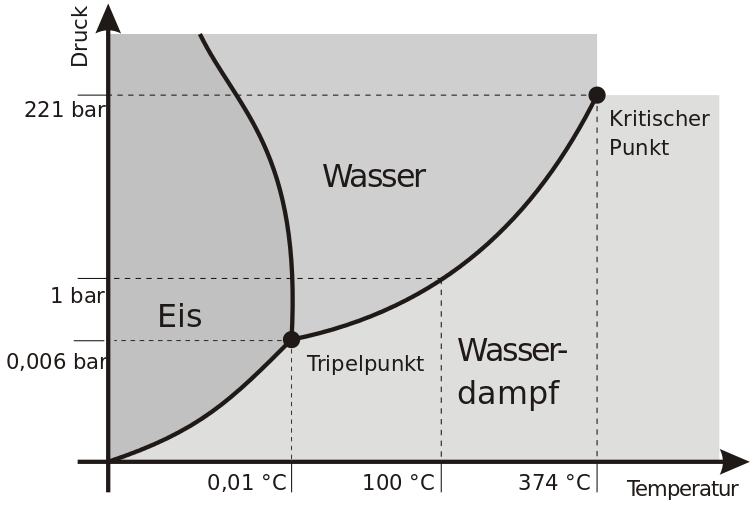
\includegraphics[width=0.7\textwidth]{img/ptwasser2}
			\caption{p-T-Zustandsdiagramm von Wasser \cite{Wikipedia.2019}}
			\label{fig:ptwasser}
		\end{figure}
		\FloatBarrier
		%Ende}
		
		\item \textit{Was sind reduzierte thermodynamische Größen und in welchem Zusammenhang stehen diese zum Korrespondenzprinzip und zu generalisierten Zustandsgleichungen?} 
		
		\textbf{Reduzierte Größen:}\\
		Als reduzierte, thermodynamische Größen bezeichnet man definierte Größen, welche das Verhältnis der jeweiligen thermodynamischen Größe zu ihrem kritischen Wert darstellen \cite{Foth.2008}. 
		\begin{flalign}
			\vartheta &=\frac{T}{T_k}
		\end{flalign}
		\begin{flalign}
		\pi &=\frac{p}{p_k}
		\end{flalign}
			\begin{flalign}
		\varphi &=\frac{V}{V_k}
		\end{flalign}
		\newpage
		Das Korrespondenzprinzip beschreibt dabei ein bestimmtes Verhältnis zu einer alten Theorie, wie der ursprünglichen \textsc{Van-der-Waals}-Gleichung und einer neueren Theorie, wie zum Beispiel der angepassten \textsc{Van-der-Waals}-Gleichung mit reduzierten, thermodynamischen Größen (siehe \eqref{gl1},\eqref{gl2}).
		\begin{flalign}
		\label{gl1}
		\left(p+\frac{a}{{V_m}^2}\right)*\left(V_m-b\right)&= R*T
		\end{flalign}
		\begin{flalign}
			\label{gl2}
			\left(\pi+\frac{3}{\varphi^2}\right)\left(3*\varphi-1\right) &= 8*\vartheta
		\end{flalign}
		Mit der neueren Theorie wird kein Widerspruch zur alten Theorie ausgedrückt. Jedoch beschreibt die ältere Theorie dabei lediglich einen eingeschränkteren Gültigkeitsbereich, als es die neue, erweiterte Theorie kann.
		
		\item \textit{Warum kann vom Manometerstand einer Flüssiggas-Druckflasche nicht auf ihren Füllstand geschlossen werden? Wie wird hier typischerweise der Füllstand überprüft?}
		
		Allein über den Druck lässt sich die Füllmenge des Gases in der Druckflasche nicht bestimmen, da der Druck des Gases eine Funktion der Temperatur darstellt. Den Füllstand Flasche sollte man aus diesem Grund über die Masse bestimmen. Dafür wird jedoch auch das Leergewicht der Gasflasche benötigt.
		 
		\item \textit{Übertragen Sie ihre experimentell aufgenommene Druck-, Temperatur-, Volumen- und Höhenwerte in ein Datenauswerte-Programm, z.B. Excel. Führen Sie die Druckkorrektur aus und bestimmen Sie die Stoffmenge n gemäß Abschnitt 5.2.}
		
		siehe Abschnitt \ref{sec:ergebnisse}
	
		\item \textit{Erstellen und beschreiben Sie ein (pV/R*T)-p-Zustandsdiagramm und ein p-Vm-Zustandsdiagramm mit allen von Ihnen experimentell aufgenommenen Isothermen.}
			\begin{figure}[h!]
				\begin{center}
					\resizebox{0.4\textwidth}{!}{
						\begin{tikzpicture}[trim axis left, trim axis right]
						\begin{axis}[
						axis lines = left,
						width = 15cm,
						height = 11cm,
						xmin = 1000,
						xmax = 5000,
						ymin = 0,
						ymax = 4.0e-6,
						%	ytick = {-4.5,-4,...,-1},
						%	xtick = {-10,-9,...,20},
						ylabel={Stoffmenge in \si{\kilo \mol}},
						%y label style={at={(0,0.5)}},
						xlabel={Druck in \si{\kilo \pascal}},
						legend style={at={(0.75,0.6)},anchor=west},
						%	y dir = reverse,
						]
							\addplot [color=black, mark=*] coordinates{(1715.593552,2.72274396362054E-06) (1783.392808,2.68882795533436E-06) (1863.058648,2.66110146754721E-06) (1929.457656,2.60283462993869E-06) (2020.123496,2.56484016186231E-06) (2108.789336,2.51007592756214E-06) (2194.588592,2.43805532153746E-06) (2296.121016,2.3686480161337E-06) (2406.053688,2.29112594210156E-06) (2513.31928,2.19382888776975E-06) (2619.251952,2.07845046782657E-06) (2676.65096,1.91159838296396E-06) (2680.717048,1.70177980725278E-06) (2681.98264,1.48976032946659E-06) (2683.64848,1.27773055993616E-06) (2686.180904,1.06578024163015E-06) (2698.113576,8.56411758327314E-07) (2705.31308,7.51359842018043E-07) (2721.779416,6.47942672661136E-07) (2735.97892,5.42769154175439E-07) (3482.712088,5.52726098997967E-07) (4850.045008,6.73513368550911E-07) };
							
								\addplot [color=brown, mark=*] coordinates{(1809.726968,2.7804213411711E-06) (1884.392808,2.75037934870788E-06) (1965.791816,2.71817608552944E-06) (2049.591072,2.67660140414793E-06) (2147.256912,2.63919543607175E-06) (2242.789336,2.58432602424148E-06) (2345.32176,2.52230748179461E-06) (2460.121016,2.45678630655597E-06) (2585.786856,2.38364474374417E-06) (2717.586112,2.29637895977425E-06) (2859.98512,2.19700645558369E-06) (3001.65096,2.07524921768687E-06) (3146.583632,1.93373441118826E-06) (3285.116056,1.7665108787914E-06) (3358.781896,1.54810571358699E-06) (3365.047488,1.29249467117537E-06) (3368.113576,1.03493786983214E-06) (3375.713328,9.07613949696203E-07) (3385.512584,7.8021311549773E-07) (3416.97892,6.56220612245125E-07) (4690.31184,7.38623530038516E-07) (4910.178424,7.5438809944548E-07) };
						
						\addplot [color=blue, mark=*] coordinates{(1900.726968,2.82986389056993E-06) (1983.259392,2.80510379547671E-06) (2070.791816,2.77475575149913E-06) (2162.32424,2.73643762679967E-06) (2265.256912,2.69807030512243E-06) (2372.789336,2.64951422860374E-06) (2488.455176,2.59342488168714E-06) (2619.254432,2.53476005779796E-06) (2758.65344,2.46430357054391E-06) (2911.719528,2.38428430267054E-06) (3075.251952,2.28926736977025E-06) (3260.784376,2.18464264050977E-06) (3451.183384,2.05529345403943E-06) (3638.715808,1.8961032942985E-06) (3834.381648,1.7126254876717E-06) (3997.31432,1.48783276660308E-06) (4118.113576,1.2262361824908E-06) (4268.646,9.5329476934841E-07) (4772.845504,8.88245877395173E-07)};
						
						
						\addplot [color=red, mark=*] coordinates{(1950.726968,2.86005279815834E-06) (2031.392808,2.82940475063201E-06) (2122.925232,2.80126871402144E-06) (2217.591072,2.76361761870505E-06) (2327.123496,2.7295243980632E-06) (2439.65592,2.68267094332018E-06) (2561.588592,2.62896608204171E-06) (2696.254432,2.56951875046436E-06) (2848.786856,2.50604444984312E-06) (3011.31928,2.42827046060589E-06) (3181.98512,2.33262921860477E-06) (3380.784376,2.23052733054079E-06) (3594.450216,2.10799718602376E-06) (3819.849224,1.96016137793788E-06) (4049.64848,1.78121418170423E-06) (4271.447736,1.56564273857082E-06) (4369.513824,1.44142881083993E-06) (4476.446496,1.31262586068794E-06) (4593.912832,1.17868664165102E-06) (4800.512584,1.05573868155471E-06) };
						
						
						\legend{Messreihe 1: T=\SI{303,15}{\kelvin}, Messreihe 2: T=\SI{313,15}{\kelvin}, Messreihe 3: T=\SI{323,15}{\kelvin}, Messreihe 3: T=\SI{323,15}{\kelvin}, Messreihe 4: T=\SI{328,15}{\kelvin}}
						\end{axis}
						\end{tikzpicture}
					}
					\caption{Berechnete Stoffmengen in Abhängigkeit vom Druck der Messreihen 1 bis 4 von \ce{SF6}}
					\label{dia:pvrt}
				\end{center}
			\end{figure}
			\FloatBarrier
			
			\newpage
			In Abb. \ref{dia:pvrt} sind die berechneten Stoffmengen über den vorherrschenden Druck aufgetragen. Zu sehen ist, dass die überkritischen Messreihen 3 und 4 einen deutlicher ausgeprägten, linearen Verlauf aufweisen, als die unterkritischen Messreihen 1 und 2. Zudem nähern sich die überkritischen Messreihen deutlich stärker aneinander an, als es die unterkritischen Messreihen in ihrem Verlauf zeigen.\linebreak 
			Grund für diese unterschiedlichen Verläufe der Graphen lässt sich wiederholt über die Phasenübergänge erklären, bei welchen in den Messreihen 1 und 2 isobare Verläufe erkennbar sind (mehr dazu unter Abschnitt \ref{sec:ergebnisse}).
			
	\begin{figure}[h!]
	\begin{center}
		\resizebox{0.4\textwidth}{!}{
			\begin{tikzpicture}[trim axis left, trim axis right]
			\begin{axis}[
			axis lines = left,
			width = 15cm,
			height = 11cm,
			xmin = 0,
			xmax = 1,
			ymin = 1500,
			ymax = 5000,
			%	ytick = {-4.5,-4,...,-1},
			%	xtick = {-10,-9,...,20},
			ylabel={Druck in \si{\kilo \pascal}},
			y label style={at={(-0.05,0.5)}},
			xlabel={molares Volumen in \si{ \liter \per \kilo \mol}},
			legend style={at={(0.75,0.6)},anchor=west},
			%	y dir = reverse,
			]
			\addplot [color=black, mark=*] coordinates{(0.935094018386433,1715.593552) (0.888339317467111,1783.392808) (0.841584616547789,1863.058648) (0.794829915628468,1929.457656) (0.748075214709146,2020.123496) (0.701320513789824,2108.789336) (0.654565812870503,2194.588592) (0.607811111951181,2296.121016) (0.561056411031859,2406.053688) (0.514301710112538,2513.31928) (0.467547009193216,2619.251952) (0.420792308273894,2676.65096) (0.374037607354573,2680.717048) (0.327282906435251,2681.98264) (0.280528205515929,2683.64848) (0.233773504596608,2686.180904) (0.187018803677286,2698.113576) (0.163641453217625,2705.31308) (0.140264102757965,2721.779416) (0.116886752298304,2735.97892) (0.093509401838643,3482.712088) (8.18207266088129E-02,4850.045008) };
			
			\addplot [color=brown, mark=*] coordinates{(0.935094018386433,1809.726968) (0.888339317467111,1884.392808) (0.841584616547789,1965.791816) (0.794829915628468,2049.591072) (0.748075214709146,2147.256912) (0.701320513789824,2242.789336) (0.654565812870503,2345.32176) (0.607811111951181,2460.121016) (0.561056411031859,2585.786856) (0.514301710112538,2717.586112) (0.467547009193216,2859.98512) (0.420792308273894,3001.65096) (0.374037607354573,3146.583632) (0.327282906435251,3285.116056) (0.280528205515929,3358.781896) (0.233773504596608,3365.047488) (0.187018803677286,3368.113576) (0.163641453217626,3375.713328) (0.140264102757965,3385.512584) (0.116886752298304,3416.97892) (9.58471368846093E-02,4690.31184) (9.35094018386433E-02,4910.178424) };
			
			\addplot [color=blue, mark=*] coordinates{(0.935094018386433,1900.726968) (0.888339317467111,1983.259392) (0.841584616547789,2070.791816) (0.794829915628468,2162.32424) (0.748075214709146,2265.256912) (0.701320513789824,2372.789336) (0.654565812870503,2488.455176) (0.607811111951181,2619.254432) (0.561056411031859,2758.65344) (0.514301710112538,2911.719528) (0.467547009193216,3075.251952) (0.420792308273894,3260.784376) (0.374037607354573,3451.183384) (0.327282906435251,3638.715808) (0.280528205515929,3834.381648) (0.233773504596608,3997.31432) (0.187018803677286,4118.113576) (0.140264102757965,4268.646) (0.116886752298304,4772.845504) };
			
			
			\addplot [color=red, mark=*] coordinates{(0.935094018386433,1950.726968) (0.888339317467111,2031.392808) (0.841584616547789,2122.925232) (0.794829915628468,2217.591072) (0.748075214709146,2327.123496) (0.701320513789824,2439.65592) (0.654565812870503,2561.588592) (0.607811111951181,2696.254432) (0.561056411031859,2848.786856) (0.514301710112538,3011.31928) (0.467547009193216,3181.98512) (0.420792308273894,3380.784376) (0.374037607354573,3594.450216) (0.327282906435251,3819.849224) (0.280528205515929,4049.64848) (0.233773504596608,4271.447736) (0.210396154136947,4369.513824) (0.187018803677287,4476.446496) (0.163641453217626,4593.912832) (0.140264102757965,4800.512584) };
			
			\legend{Messreihe 1: T=\SI{303,15}{\kelvin}, Messreihe 2: T=\SI{313,15}{\kelvin}, Messreihe 3: T=\SI{323,15}{\kelvin}, Messreihe 3: T=\SI{323,15}{\kelvin}, Messreihe 4: T=\SI{328,15}{\kelvin}}
			\end{axis}
			\end{tikzpicture}
		}
		\caption{Druck in Abhängigkeit vom molaren Volumen der Messreihen 1 bis 4 von \ce{SF6}}
		\label{dia:pvm}
	\end{center}
\end{figure}
\FloatBarrier
 In Abb. \ref{dia:pvm} ist der Druck in Abhängigkeit vom molaren Volumen aufgetragen. Der Verlauf der Graphen lässt sich hierbei analog auf die schon beschriebene Abb. \ref{dia:isotherme} beziehen. Der Unterschied beider Darstellungen lässt sich auf die Normierung des Volumens auf die berechnete Stoffmenge erklären.

\item \textit{Berechnen Sie den zweiten Virialkoeffizient B mit Hilfe des aus Gleichung 10 erhaltenen Geradenanstiegs b und dem unter Kapitel 5.2 ermittelten Wert der Stoffmenge. Vergleichen Sie den berechneten Virialkoeffizienten B mit Literaturwerten.}
\begin{flalign}
p*V_m&= R*T+B(T)*p\\
\frac{p*V}{R*T}&=n+\frac{B(T)*p*n}{R*T} = a+b*p\\
a+b*p	&=n+\frac{B(T)*p*n}{R*T}\\[1mm] \tag{a=n}
b&=\frac{n}{p}+\frac{B(T)*n}{R*T}-\frac{a}{p}\\
b 				  &= \frac{B(T)*n}{R*T}	\\[1mm]
B(T)			&=\frac{b*R*T}{n}
\end{flalign}

\begin{flalign}
B(T)			&=\frac{b*R*T}{n}\\
B(\SI{323,15}{\kelvin})	&=\frac{\SI{-3,84}{\kmol \per \kilo \pascal}*\SI{8,314}{\joule \per \mole \per \kelvin}*\SI{303,15}{\kelvin}}{\SI{4,28E-06}{\kmol}} =\underline{\SI{ -289	}{\raiseto{3} \centi \meter \per \mole}}	\\		
\end{flalign}
% Table generated by Excel2LaTeX from sheet 'Daten'
\begin{table}[h!]
	\centering
	\caption{experimentell ermittelte Virialkoeffizienten der Messreihen 3 und 4 gegenübergestellt mit Literaturwerte \cite{Lide.1994}}
	%\resizebox{10.5cm}{!}{
		\begin{tabulary}{\textwidth}{C|C|C|C}
			\hline
			\textbf{M3: $T=\SI{323,15}{\kelvin}$}&\textbf{M4: $T=\SI{328,15}{\kelvin}$}&\textbf{Literaturwert \SI{300}{\kelvin}}&\textbf{Literaturwert \SI{350}{\kelvin}}\\
			\hline
			\SI{-289}{\raiseto{3} \centi \meter \per \mole}&	\SI{-274}{\raiseto{3} \centi \meter \per \mole} &	\SI{-275}{\raiseto{3} \centi \meter \per \mole}&	\SI{-190}{\raiseto{3} \centi \meter \per \mole}\\
			\label{tab:Koeffizienten}%
	\end{tabulary}
%}
\end{table}%
\FloatBarrier

Die Virialkoeffizienten der Messreihen 3 und 4 wichen zum Teil ziemlich stark von den Literaturwerten \cite{Lide.1994} ab. Zwar ist die Tendenz, dass mit steigender Temperatur der Wert für den Virialkoeffizient sinkt zu erkennen, jedoch erscheinen die in den Werten selbst vergleichsweise hoch. Grund hierfür könnten Messungenauigkeiten für die Höhe $h$ in der Druckkorrektur sein \mbox{(siehe Abschnitt \ref{sec:fehler})}.

\item \textit{Vergleichen Sie die experimentellen Werte mit theoretisch berechneten Berechnungsergebnissen der CEOS-van-der-Waals und CEOS-PENG-ROBINSONGleichung aus dem PC-Softwareprogramm ZUST.}  
\begin{figure}[h!]
\centering
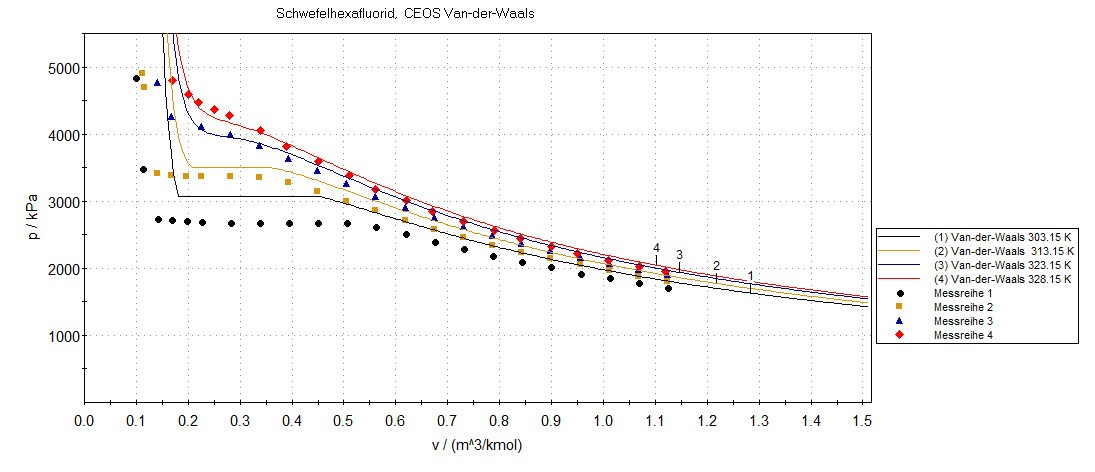
\includegraphics[width=0.85\textwidth]{img/VDW}
\caption{Messdaten mit CEOS-\textsc{Van-der-Waals}-Dampfdruckkurven}
\label{fig:vdW}
\end{figure}
\FloatBarrier
%Ende
\begin{figure}[h!]
	\centering
	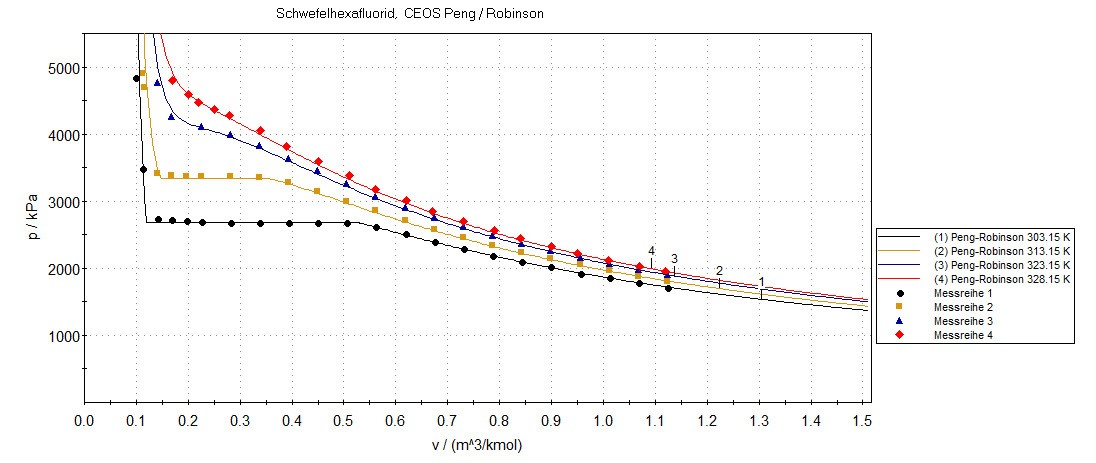
\includegraphics[width=0.85\textwidth]{img/PR}
	\caption{Messdaten mit CEOS-\textsc{Peng-Robinson}-Dampfdruckkurven}
	\label{fig:pr}
\end{figure}
\FloatBarrier
%Ende
In Abb. \ref{fig:vdW} und Abb. \ref{fig:pr} sind aufgenommen Messdaten Druck und molare Volumen gegeneinander aufgetragen. Weiterhin sind in den dargestellten Diagrammen Dampfdruckkurven zwei verschiedener Berechnungsmodell eingezeichnet, welche mit dem Programm \textsc{ZUST} berechnet wurden \cite{zust}. Verwendet wurden die Berechnungsmodelle für die \textsc{Van-der-Waals}-Gleichung (Abb. \ref{fig:vdW}) und der \textsc{Peng-Robinson}-Gleichung (Abb. \ref{fig:pr}).\\
Im Vergleich der beiden Graphen sieht man sofort, dass die \textsc{Peng-Robinson}- Gleichung deutlich besser die aufgenommen Messdaten der Temperaturbereiche erfasst, als es die \textsc{Van-der-Waals}-Gleichung kann. Die \textsc{Van-der-Waals}-Gleichung scheint lediglich im bei den überkritischen Isothermen mit der \textsc{Peng-Robinson}- Gleichung mithalten zu können. Das erklärt sich vermutlich aus dem Zusammenhang heraus, dass sich die \textsc{Van-der-Waals}-Gleichung näher aus dem idealen Gasgesetz ableitet als die \textsc{Peng-Robinson}-Gleichung. So erklärt sich, dass die \textsc{Van-der-Waals}-Gleichung die Messdaten erst unter "`idealeren"' Bedingungen ihren Gültigkeitsbereich ausbildet. Diese "`idealeren"' Bedingungen werden dabei durch höhere Temperaturen , kleinere Drücke und große Volumina ausgedrückt.\\
Müssten man also bestimmte Verläufe von \ce{SF6}-Isothermen voraussagen, so erscheint die \textsc{Peng-Robinson}-Gleichung als qualitativ hochwertiger. 

\end{enumerate}
















\section{Zusammenfassung und Fazit}
\label{sec:zusammenfassung}
%Abschließende Zusammenfassung bezüglich der angewendeten Methode, der
%erzielten experimentellen-analytischen Ergebnisse und dem Ergebnis aus der
%Diskussion und Einordnung.
%- Abschließende Reflektion zwischen angestrebten Versuchsziel und den erzielten
%Ergebnissen.
%- Gegebenenfalls: Ausblick -> experimentelle Verbesserungsvorschläge zur Erhöhung
%der Genauigkeit, weitere experimentelle Reihen zur „noch besseren“ Lösung oder
%Erweiterung des Wissenszuwachses aus der Aufgabenstellung

\textcolor{red}{Fazit schreiben}

%Praktikumsskript, Modul ………, Versuch …….., Prof. Musterprof. 
%DIN 12345, Jahr der Veröffentlichung 
%Link der Internetseite, Zugriffsdatum 
%Buchtitel, Autor, Verlag, Veröffentlichungsjahr 

%Literaturverzeichnis Bücher
\bibliography{Literatur}
\bibliographystyle{unsrtdin}
\addcontentsline{toc}{section}{Literaturverzeichnis}



%\section*{Anhang}
\addcontentsline{toc}{section}{Anhang}
\label{sec:anhang}

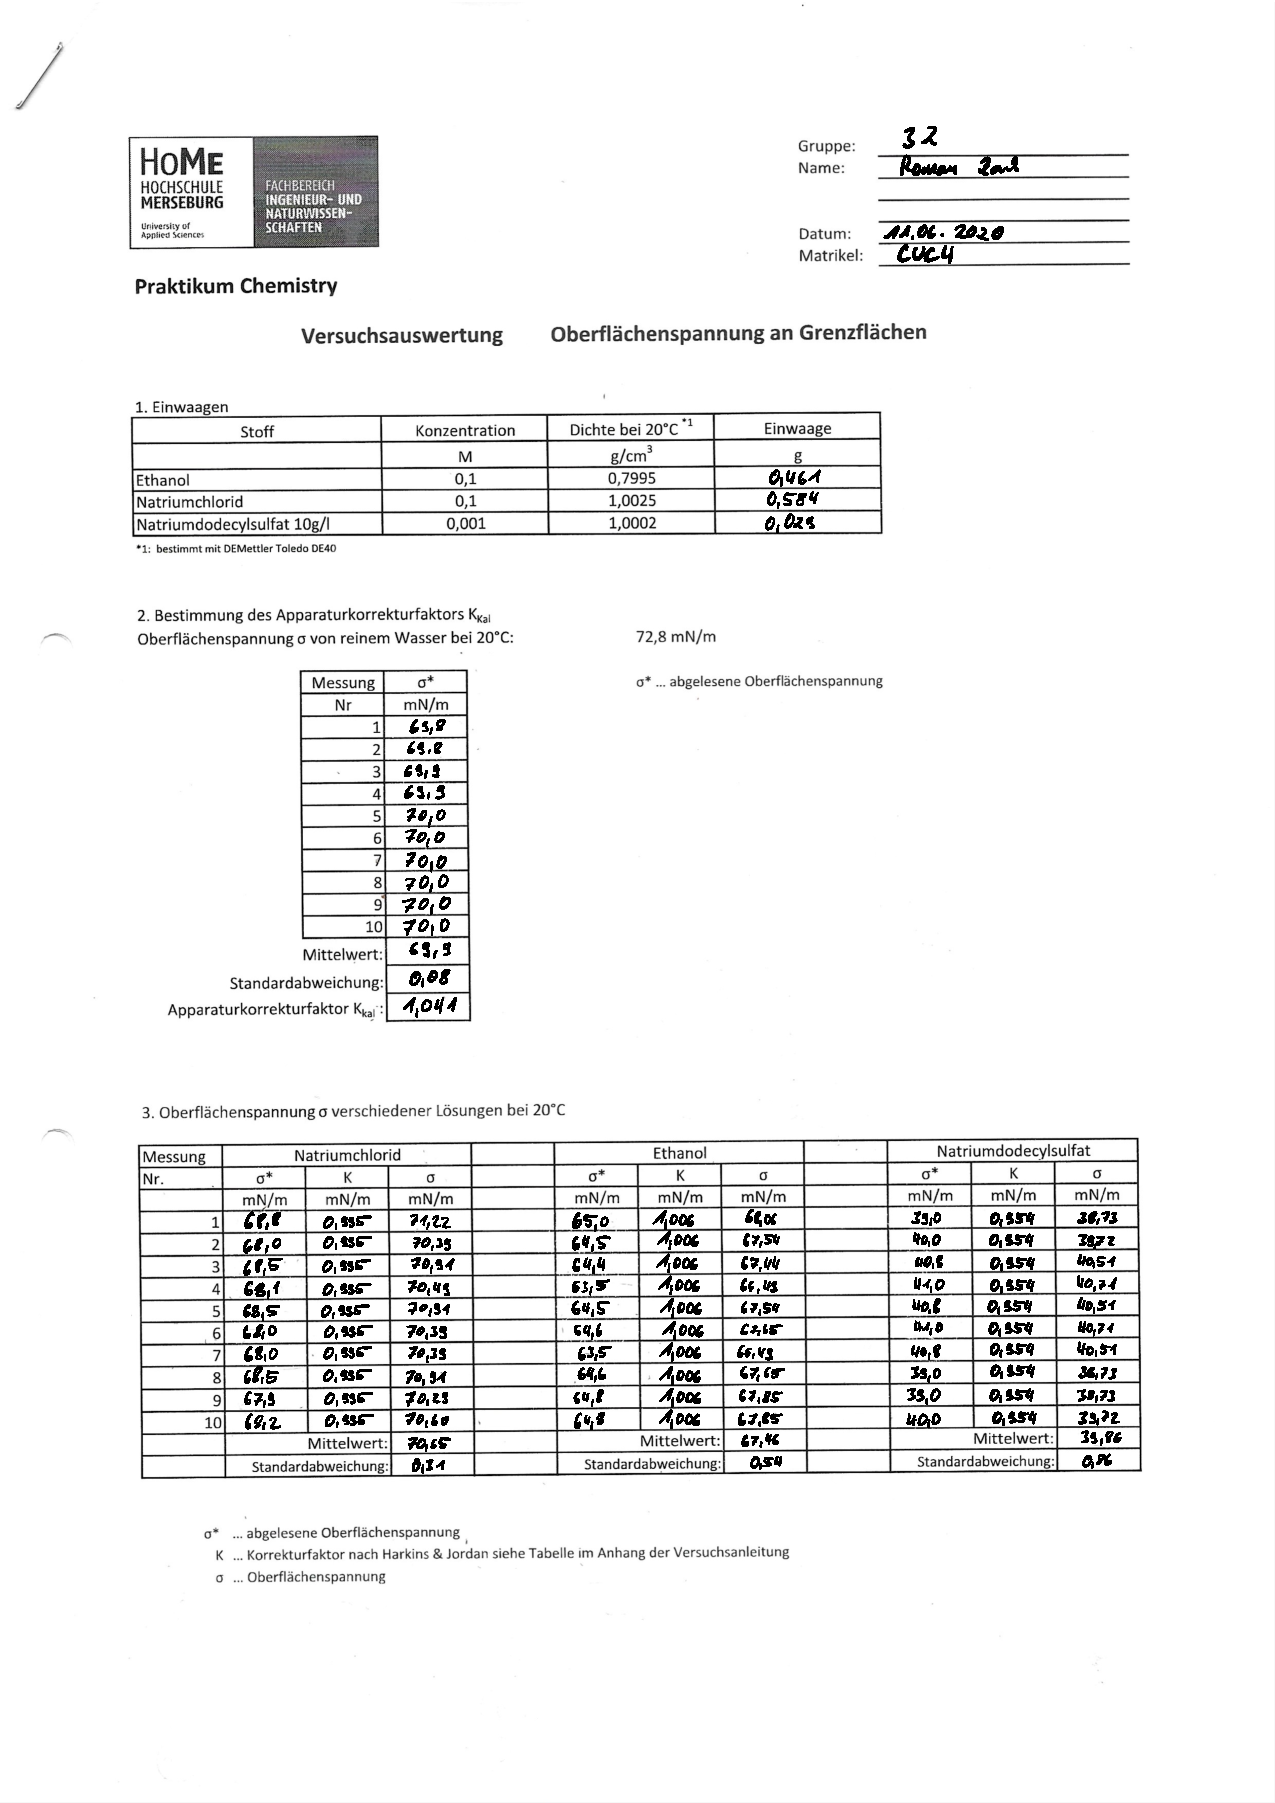
\includepdf[pages=1-2]{data/surf_data}

%\chapter*{Eidesstattliche Erklärung}
\label{erklaerung}
Hiermit versichere ich, die vorliegende Seminararbeit selbstständig und nur unter Verwendung der von mir angegebenen Quellen und Hilfsmittel verfasst zu haben. Sowohl inhaltlich als auch wörtlich entnommene Inhalte wurden als solche kenntlich gemacht. Die Arbeit hat in dieser oder vergleichbarer Form noch keinem anderem Prüfungsgremium vorgelegen. \\
\\[1.5cm]
Datum:	\hrulefill\enspace Unterschrift: \hrulefill
\\[3.5cm]
\addcontentsline{toc}{chapter}{Selbstständigkeitserklärung}

\end{document}
